% - - - - - - - - - - - - - - - - - - - - - - - - - - - - 
\subsection{PROC-01 Realización de una venta al cliente}

\begin{figure}[htbp]
	\begin{center}
		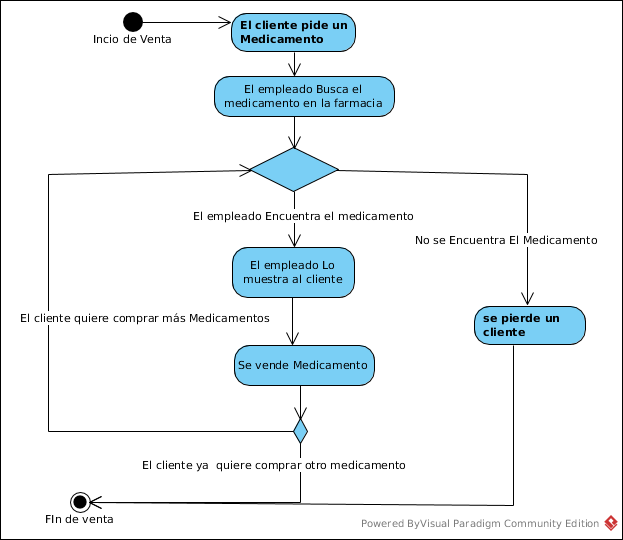
\includegraphics[width=.7\textwidth]{images/AS-TOprocVenta}
		\caption{PROC-01 Realización de una venta al cliente}
		\label{fig:proceso1}
	\end{center}
\end{figure}

\begin{description}
	\item[Descripción:] Ocurre cuando llega un cliente a la farmacia en busca de un medicamento que quiere comprar, el empleado de planta se tarda aproximadamente 7min en buscar un medicamento,una vez que este se encuentra se le muestra al cliente y se vende. 
	\item[Entradas:] \cdtEmpty
        \begin{itemize}
			\item Cliente
			\item Dinero
        \end{itemize}
	\item[Salidas:] \cdtEmpty
        \begin{itemize}
			\item Medicamento
        \end{itemize}	
    \item[Áreas de oportunidad:]la búsqueda del medicamento será mucho más rápida y eficiente, lo cual le ahorra tiempo al cliente y a la farmacia aparte de tener mejor guardados los datos de una venta.
\end{description}
